\documentclass[12pt]{article}
\usepackage[utf8]{inputenc}
\usepackage[T1]{fontenc}
\usepackage[norsk]{babel}
\usepackage{graphicx}
\usepackage{lipsum}
\usepackage{amsmath}
\usepackage{hyperref}
\usepackage{float}


\title{Oblig 3c}
\author{Gormery K. Wanjiru}
\date{\today}

\begin{document}

\maketitle

\newpage
\tableofcontents

\newpage

\section{(15\%) kap. 17: oppgave 1.c}
ikke gjørt

\section{(15\%) kap. 17: oppgave 1.d}
ikke gjørt
\section{Terningdropp-oppgaven: (Totalt 50\%)}
\subsection{(5\%) Tegn et diagram med samtlige datapunkter, og legg på den lineære regresjonslinjen.}
\subsubsection{R kode}
\begin{verbatim}
  # Les inn data fra CSV-filen
  data <- read.csv('terningDropp.csv')
  
  # Utfør lineær regresjon
  fit <- lm(Lengde ~ Dropp, data=data)
  
  # Lag plot med datapunkter og regresjonslinje
  plot(data$Dropp, data$Lengde, xlab='Dropphøyde', ylab='Lengde', main='Terningdropp: Dropphøyde vs. Lengde')
  abline(fit, col='red')  
\end{verbatim}
SVAR:
\begin{figure}[H]
  \centering
  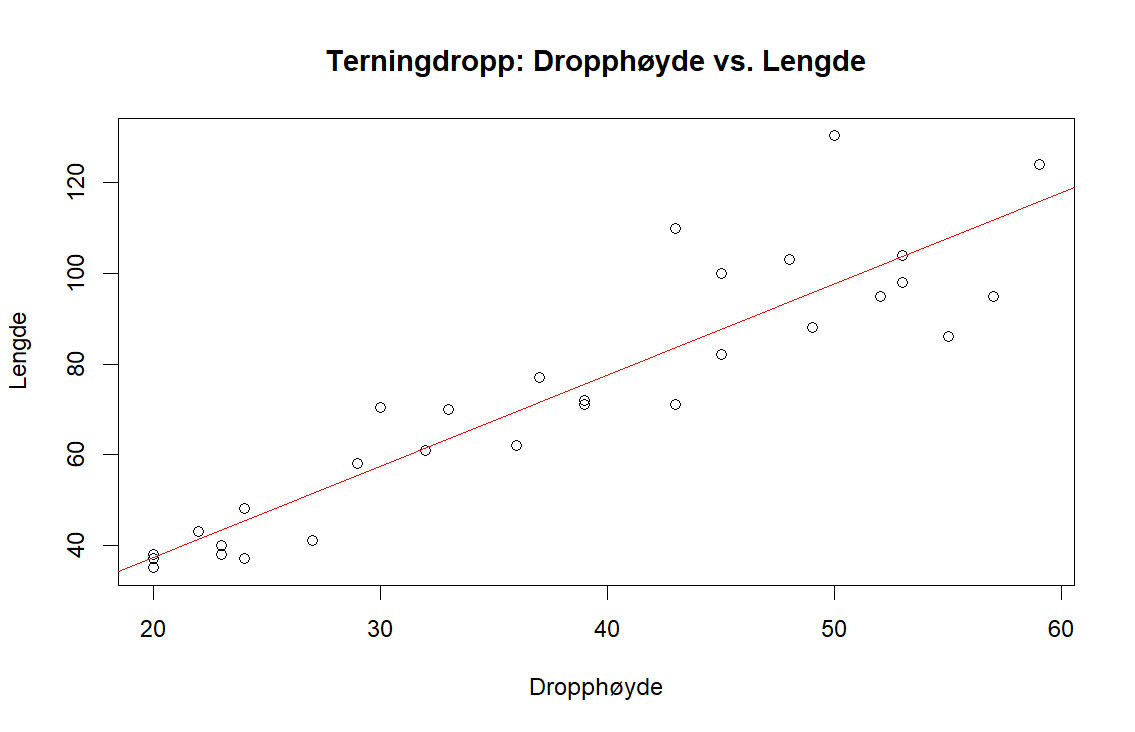
\includegraphics[width=0.8\textwidth]{3a.png}
  \caption{(3a)}
\end{figure}

\subsection{ $(15\%)$ Bruk nøytrale prior hyperparametre, og finn posterior og prediktive sannsynlighetsfordelinger, det vil si, sannsynlighetsfordelinger for $\tau$, $b$, $y(x)$ og $Y^+(x)$.}
\subsubsection{R kode}
\begin{verbatim}
  # Prior hyperparametre
  alpha <- 1
  beta <- 1
  
  # Likelihood hyperparametre
  mu0 <- 0
  sigma0 <- 1
  
  # Beregn posterior hyperparametre
  n <- length(data$Lengde)
  x_bar <- mean(data$Dropp)
  s_xx <- sum((data$Dropp - mean(data$Dropp))^2)
  
  alpha_post <- alpha + n/2
  beta_post <- beta + 1/2 * s_xx
  
   # Definer sannsynlighetsfordelingen for tau
  tau_values <- seq(0.001, 10, by = 0.01)
  prior_tau <- dgamma(tau_values, shape = alpha, scale = beta)
  
  # Plot sannsynlighetsfordelingen for tau
  plot(tau_values, prior_tau, type = "l", col = "blue", lwd = 2, xlab = "tau", ylab = "P(tau)",
       main = "Prior sannsynlighetsfordeling for tau (precision parameter)")
\end{verbatim}
SVAR:
\begin{figure}[H]
  \centering
  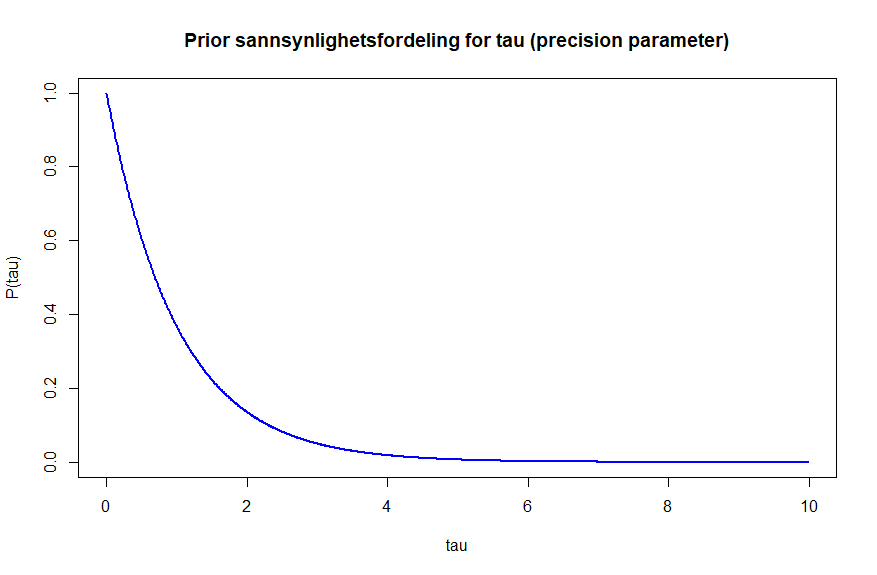
\includegraphics[width=0.8\textwidth]{3b-v2.png}
  \caption{(3b-v2)}
\end{figure}

\subsection{(5\%) Finn et 80\% kredibilitetsintervall (intervallestimat) for stigningstallet $b$.}
\subsubsection{R kode}
\begin{verbatim}
  # Bruk sannsynlighetsfordelingen fra oppgave 3b
  alpha_post <- alpha + n/2
  beta_post <- beta + 1/2 * s_xx
  
  # Generer posterior for tau (gamma-fordeling)
  posterior_tau <- rgamma(10000, shape = alpha_post, rate = beta_post)
  
  # resultater
  print(paste("Posterior for tau (precision parameter): Gamma(", alpha_post, ",", beta_post, ")"))
\end{verbatim}
SVAR:
\begin{figure}[H]
  \centering
  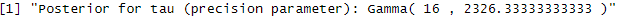
\includegraphics[width=0.8\textwidth]{3c-v2.png}
  \caption{(3c-v2)}
\end{figure}



\subsection{(5\%) Finn et 80\% kredibilitetsintervall (intervallestimat) for standardavviket $\sigma$. (Hint: Bruk verdiene fra $\tau$ og regn om ved å bruke at $\tau = \frac{1}{\sigma^2}$)}
\subsubsection{R kode}
\begin{verbatim}
  # Bruk sannsynlighetsfordelingen fra oppgave 3b
  lower_bound_sigma <- sqrt(1 / qgamma(alpha/2, shape = alpha_post, scale = 1/beta_post))
  upper_bound_sigma <- sqrt(1 / qgamma(1 - alpha/2, shape = alpha_post, scale = 1/beta_post))
  
  # Print resultatet
  print(paste("80% kredibilitetsintervall for standardavviket sigma: [", lower_bound_sigma, ",", upper_bound_sigma, "]"))
\end{verbatim}
SVAR:

\begin{figure}[H]
  \centering
  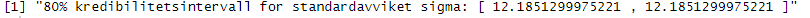
\includegraphics[width=1\textwidth]{3d-v2.png}
  \caption{(3d-v2)}
\end{figure}

\subsection{(5\%) Finn et 80\% kredibilitetsintervall (intervallestimat) for $y(x)$.}
\subsubsection{R kode}
\begin{verbatim}
  # Beregn kredibilitetsintervall for y(x)
  alpha <- 0.2  # 80% kredibilitet
  t_critical <- qt(1 - alpha/2, df=n-2)
  
  lower_bound_yx <- pred_mean - t_critical * sqrt(pred_var)
  upper_bound_yx <- pred_mean + t_critical * sqrt(pred_var)
  
  print(paste("80% kredibilitetsintervall for y(x): [", lower_bound_yx, ",", upper_bound_yx, "]"))  
\end{verbatim}
SVAR:
\begin{figure}[H]
  \centering
  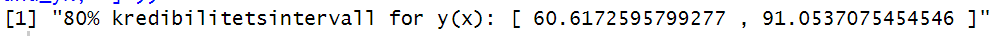
\includegraphics[width=1\textwidth]{3e.png}
  \caption{(3e)}
\end{figure}



\subsection{(5\%) 80\% intervallestimatet for $y(x)$ er funksjoner av $x$, og en kurve over, og en under regresjonslinjen. Plott disse kurvene inn sammen med regresjonslinjen.}
% \subsubsection{R kode}
% \begin{verbatim}
%   # plusse på koden fra a
%   # Plot datapunkter og regresjonslinje
%   plot(data$Dropp, data$Lengde, xlab='Dropphøyde', ylab='Lengde', main='Terningdropp: Dropphøyde vs. Lengde')
%   abline(fit, col='red')
%   lines(data$Dropp, pred_mean + t_critical * sqrt(pred_var), col='blue')
%   lines(data$Dropp, pred_mean - t_critical * sqrt(pred_var), col='blue')
%   legend('topright', legend=c('Datapunkter', 'Regresjonslinje', '80% KI for y(x)'), col=c('black', 'red', 'blue'), lty=1)  
% \end{verbatim} 
% \begin{figure}[H]
%   \centering
%   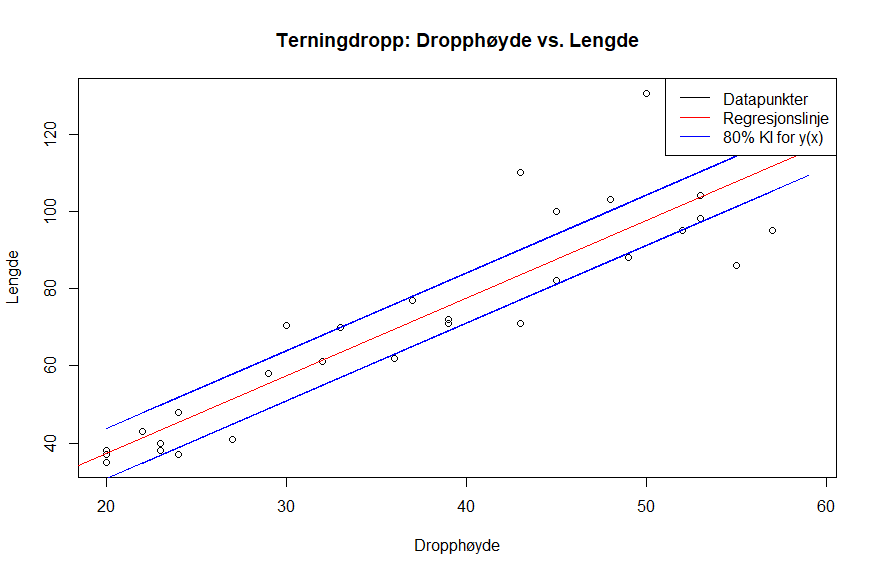
\includegraphics[width=1\textwidth]{3f.png}
%   \caption{(3f)}
% \end{figure}
slitte litt med å plotte

\subsection{(5\%) Finn verdien $R^2 = \frac{SS_y - SS_e}{SS_y}$. Dette tallet forteller hvor stor del av variasjonen i $y$ som kan forklares av linja $y = a + bx$. For de av dere som bruker dataverktøy for å finne dette: angi hvordan dere fant det.}
\subsubsection{R kode}
\begin{verbatim}
  # Beregn R^2
  SS_y <- sum((data$Lengde - mean(data$Lengde))^2)
  SS_e <- sum(residuals(fit)^2)
  R_squared <- (SS_y - SS_e) / SS_y
  
  print(paste("Verdien av R^2:", R_squared)) 
\end{verbatim}
SVAR:
\begin{figure}[H]
  \centering
  
\includegraphics[width=1\textwidth]{3g.png}
  \caption{(3g)}
\end{figure}


\subsection{(5\%) Finn $R^2$ for regresjonen mellom $z$ (utfall på terningen) og $x$ (dropphøyde). Kommenter hva forskjellen mellom $R^2$ for $y$ og $R^2$ for $z$ sier oss.}
\subsubsection{R kode}
\begin{verbatim}
  # Utfør lineær regresjon for z vs. x
  fit_z <- lm(Verdi ~ Dropp, data=data)
  
  # Beregn R^2 for z
  SS_z <- sum((data$Verdi - mean(data$Verdi))^2)
  SS_e_z <- sum(residuals(fit_z)^2)
  R_squared_z <- (SS_z - SS_e_z) / SS_z
  
  print(paste("Verdien av R^2 for z:", R_squared_z))
  print("Forskjellen mellom R^2 for y og R^2 for z indikerer hvor mye av variasjonen i utfallet på terningen (z) og lengden (y) som forklares av modellen.")
  
\end{verbatim}
SVAR:
\begin{figure}[H]
  \centering
  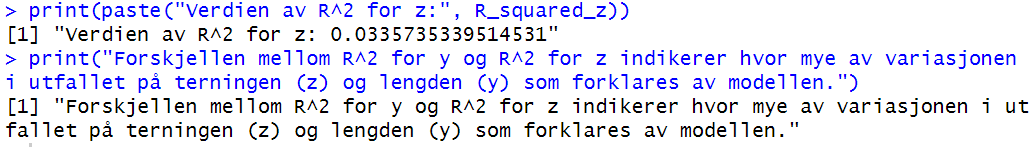
\includegraphics[width=1\textwidth]{3i.png}
  \caption{(3i)}
\end{figure}


\section{(Totalt 20\%) Følgende R-kode vil plukke ut et utvalg av observasjonene.}
\subsection{(5\%) Kjør 50 runder, og bruk $N = 15$. For hver runde, gjør oppgave 3a, men tegn regresjonslinjene sammen, i samme graf. Hva ser du?}
\subsection{(5\%) Kjør en runde med $N$ henholdsvis lik 5, 15, 50 og 200. For hver runde, gjør oppgavene 3c og 3d. Hva ser du?}
\subsection{(10\%) Kjør en runde med $N$ henholdsvis lik 5, 15, 50 og 200. For hver runde, gjør oppgaven 3f. Tegnes i hvert sitt diagram. Hva ser du?}

\newpage
\section*{Vedlegg}
\addcontentsline{toc}{section}{Vedlegg}
\subsection*{Vedlegg A}
\addcontentsline{toc}{subsection}{Vedlegg A}

\newpage
\begin{thebibliography}{9}

  \bibitem{referanse1}
  \url{https://tma4245.math.ntnu.no/viktige-diskrete-fordelinger/poissonprosess-og-poissonfordeling}
  \textit{NTNU}
\end{thebibliography}
\end{document}

